
\section{DOFA Model}
\label{sec:dofa}

\begin{figure}[h]
	\centering
	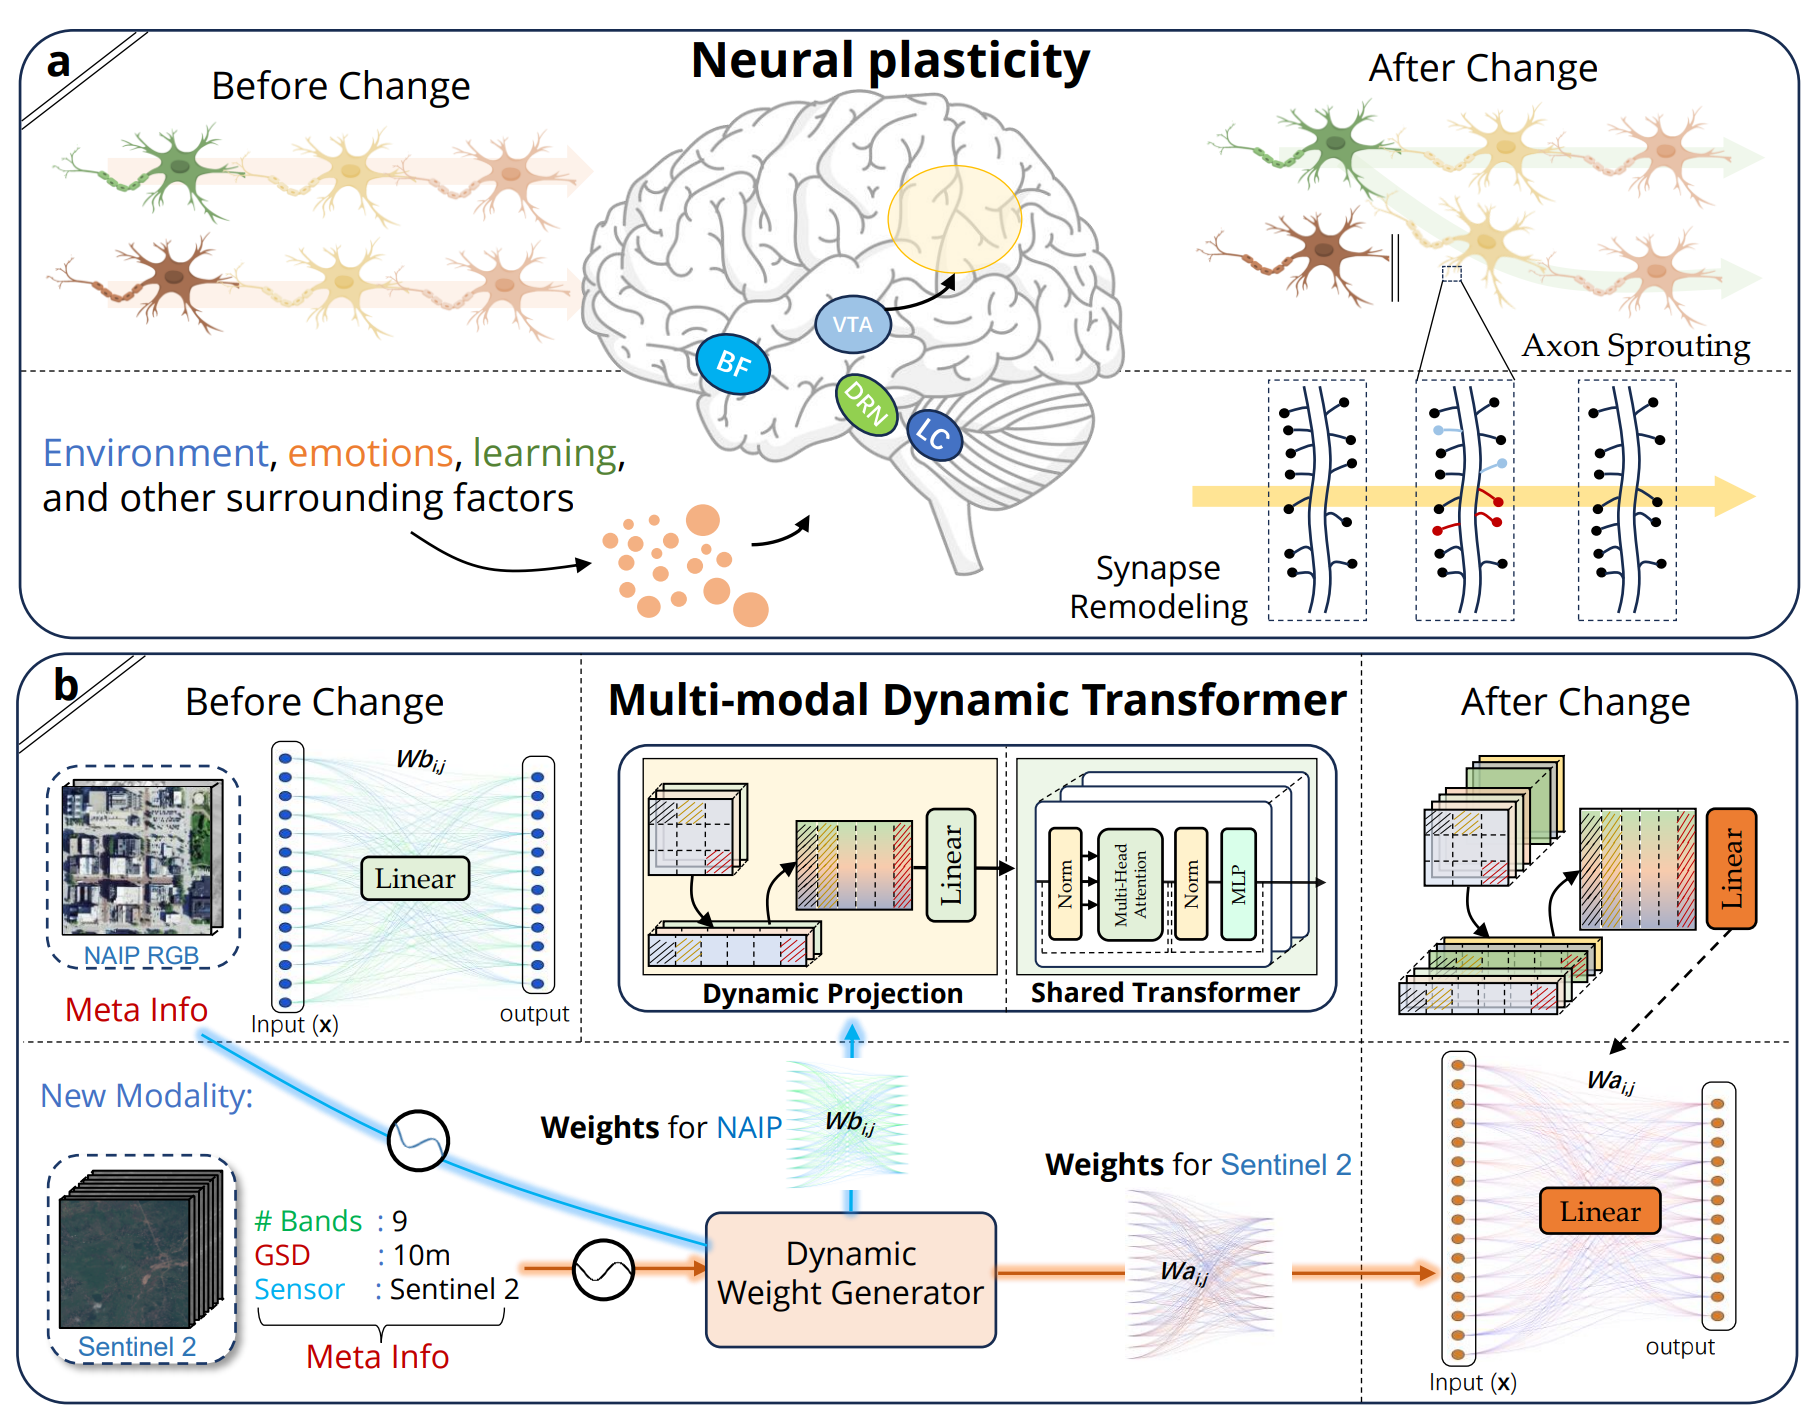
\includegraphics[width=\columnwidth]{images/dofa-concept.png}
	\caption{Visualization from the original paper \cite{dofa}. Shows the inspiration for neural plasticity from the human brain and it's application for the DOFA architecture.}
	\label{fig:dofa-concept}
\end{figure}

'DOFA' stands for \emph{'Dynamic-One-For-All'} model, inspired by the concept of neural plasticity from brain science. The main goal is to integrate various data modalities into a single framework, adaptively adjusting to different sensor inputs without needing separate models for each sensor type. This means that the model adjusts weights based on the varying wavelengths of the input data. The training process resembles that of a single large transformer model.

The authors used data from \emph{different sources and sensors} including Landsat, Sentinels, MODIS, EnMAP, Gaofen, and NAIP, which are representative of a large range of spectral bands, resolutions, and imaging types. DOFA is trained using masked images and predicting the missing patches to learn meaningful representations on unlabeled data. It uses \emph{pre-trained models} that were trained on ImageNet to enhance training efficiency and reduce training times. Additionally, as a new distillation loss is introduced to improve model performance.

The \emph{distillation loss} is derived from the concept of knowledge distillation, where we want to transfer knowledge from a larger model (e.g., trained on ImageNet), which we call the 'teacher' model to a smaller model which we call the 'student' model. The basic idea is that the student model (DOFA) is trained so that its output aligns closer to that of the teacher model. This is especially useful when it comes to data that the teacher model has already seen, which in this case refers to RGB images (for example on landscape images which are somewhat similar to remote sensing data). This setup should accelerate training convergence and enhance the overall performance. This loss is combined with the loss for image reconstruction. Together they guide the model to not only reproduce the input data correctly but also form representations that are informed by the teacher model.

The core idea of adjusting weights is through a second \emph{hypernetwork}. This secondary neural network is trained to generate weights and biases for the main network (transformer-based) to execute, based on the input data.The characteristics utilized include central wavelengths associated with each input band and their standard deviations. The hypernetwork learns during training to generate effective weights as it receives feedback on the performance of the primary network. This approach makes it possible to use tailored transformations for different modalities \emph{and} train everything in one go. The whole architecture is shown in Figure \ref{fig:dofa-concept}.

The authors claim that this approach using one foundational model \emph{reduces the computational overhead} and complexity compared to multiple specialized models. Through its multimodal training, the model should be able to handle EO tasks and data types that it hasn't seen before. This concept of multi-modality is expected to be transferable to other fields like medical image analysis and robotics.

The results in their paper show high performances in different datasets and downstream tasks compared to other approaches. The only dataset in their evaluation that is behind other approaches is the BigEarthNet for which we will provide more results.

\cite{dofa}